%------------------ About -----------------------
% McMaster Master's/Doctoral Thesis 
% LaTeX Template, Version 1.1 (07 Aug 2022)
% Works for only Double Spaced Thesis
% Compiler: pdfLaTeX
% TeX Live version: 2020 (Legacy)

% First modifications according to McMaster SGS 2016 Guideline:
% Dr. Omar Boursalie
%
% Updated according to McMaster SGS 2021 Guideline and made compatible to Overleaf:
% Asif Khan (https://www.linkedin.com/in/asif-k/)
% will occasionally update on Overleaf template page
% 
% Thanks to Sajjad Rashidiani for help in rechecking

%---------------- V1.1 --------------------------
% matched updated style format for double spacing by Mac SGS guideline (Aug 2021)
% Removed manual packages (in backup: fancyheadings, natbib) and added packages in preamble to work well in Overleaf
% Organized files, folders and renamed a few to match overall format
% Added hyperlinks and made it dynamic
% Other minor changes

% License:
% CC BY-NC-SA 4.0 (https://creativecommons.org/licenses/by-nc-sa/4.0/)

%----------------- preamble ------------------
\documentclass[letterpaper, 12pt]{report}                  % Letter paper, Times New Roman, 12pt, twoside or oneside

% new packages
\usepackage{lipsum}
%\usepackage[utf8]{inputenc}
\usepackage{comment}
\renewcommand{\contentsname}{Table of Contents} % to rename it from Contents to Table of Contents % https://tex.stackexchange.com/questions/28516/how-to-change-the-title-of-toc
\usepackage{geometry}
\usepackage[compress, numbers]{natbib} % Bibliography formatting
% \usepackage[round, sort, numbers]{natbib}
\usepackage{fancyhdr} % Header and footer styling
%\usepackage{fancyheadings} % deprecated               

%\usepackage{gscale_thesis_singlespace} % Single spaced thesis % only double spaced is formatted, you can update it easily if needed
\usepackage{gscale_thesis_doublespace} % Double spaced thesis

\usepackage{setspace}                           % Allows double spacing but skips headers/footers
% all the definitions are here

% thesis information
\halftitle{Short Title} % 60 Characters Max. Including Spaces
\title{Your Thesis Title, Which Can Be As Long As You Want On the Title Page}
\field{Your Field} % What field your thesis is in (if needed)

% your information
\author{Jane Doe}
\shortauthor{J. Doe} % Used for page header

% school information
\dept{\href{https://www.eng.mcmaster.ca/ece}{Electrical and Computer Engineering}} % Your department's name, print it using \@dept
\gschoolname{\href{https://gs.mcmaster.ca/}{School of Graduate Studies}}
\univname{\href{http://www.mcmaster.ca/}{McMaster University}} % Your university's name, print it using \@univname
\macaddress{Hamilton, Ontario, Canada}

% previous and current degrees
\prevdegreeone{BS (Computer Science and Engineering),\\ McMaster University, Hamilton, Canada}
\prevdegreetwo{BS} % Just your degree's field
\degreename{Master of Applied Science}

% date and time
\submitmonthyear{December 2022} % did not make dynamic on purpose
\submitdate{\today} % please use with caution
\copyrightyear{2022} % did not make dynamic on purpose

% Supervisor/Committee
\principaladviser{Your Supervisor} % Your Supervisor
                                % LaTeX variables for preface pages/headers
\setcounter{tocdepth}{1}                        % Limits the TOC to chapter and section names

% Additional packages
\usepackage{graphicx}                                   % Allows the inclusion of figures
\usepackage{subcaption}                               % Allows captions to be added to subfigures
\usepackage[justification=centering]{caption} % Centres caption text
\usepackage[hidelinks]{hyperref}                    % Linking to LaTeX labels and external URLs
\usepackage{array}                                        % Used for table formatting
\newcolumntype{P}[1]{>{\raggedright\let\newline\\\arraybackslash\hspace{0pt}}m{#1}}
\usepackage{booktabs}                                 % Fancy-style tables
\usepackage{longtable}                                 % Allows for tables that are more than one page long
\usepackage{float}                                         % Better figure placement control
\usepackage{enumerate}   
\usepackage[shortlabels]{enumitem}                            % Numbered lists 
\usepackage[shortcuts]{extdash}                  % Allows manual hyphenation of hypenated words
\usepackage{amsmath}                                % Non-standard math symbols
\usepackage{amsfonts}                                % Extended fonts for mathematics
\numberwithin{equation}{section}                 % Numbers equations based on their section


%----------------- Document Begins ------------------
\begin{document}

%--------------------Before Preface-------------------------
\beforepreface                                         % Half title page, title page, declaration page   
  \prefacesection{Lay Abstract}

A lay abstract of not more 150 words must be included explaining the key goals and contributions of the thesis in lay terms that is accessible to the general public.                                   % Lay Abstract
  \prefacesection{Abstract}

Abstract here (no more than 300 words)                                      % Abstract
  %\thispagestyle{empty}
\null\vfill
\begin{center}
%\textbf{Dedications}
%\linebreak
\textsl{Your Dedication \\ Optional second line}
\end{center}
\vfill
                                      % Dedication
  \prefacesection{Acknowledgements}

Acknowledgements go here.                 % Acknowledgements
  \referencepageswithnotations{notation} % Table of Contents, List of Figures, List of Tables, Notations
    %\referencepages % No notations version (choose one)???
  \prefacesection{Declaration of Academic Achievement}

Declaration of Academic Achievement go here.  % declaration of Academic Achievement

% add your new chapters here according to your text file name
%--------------------After Preface-------------------------
\afterpreface                      
  \chapter{Introduction}

Every thesis needs an introductory chapter

\lipsum[2-4]
\lipsum[2-4] \cite{popescu2014gamygdala}
        \setcounter{figure}{0}
        \setcounter{equation}{0}
        \setcounter{table}{0}
        
  \chapter{Your Chapter Title}

This is a sample chapter

\section{Referencing}
These are some sample references to GAMYGDALA~ \citep{popescu2014gamygdala} from the ``refernces.bib" file and state effects of cognition~\citep{hudlicka2002time} from the ``reference\_another.bib" file. These references are not in the same .bib file.

\section{Figures}
This is a single image figure (Figure~\ref{fig_singleenv}:

\begin{figure}[ht]
	\centering
	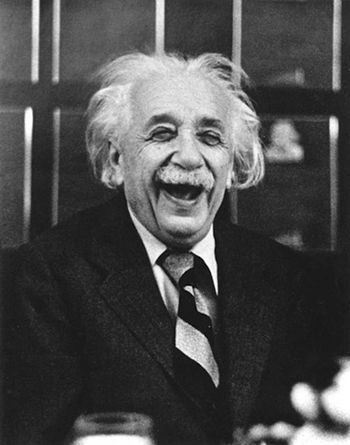
\includegraphics[width=0.6\textwidth]{figures/sample/einstein.jpeg}
	\caption[Single Figure Environment Listed Title]{This is a single figure environment}
	\label{fig_singleenv}
\end{figure}

This is a multi-image figure with a top (Figure~\ref{fig_multienv_1}) and bottom (Figure~\ref{fig_multienv_2}) aligned subfigures:

\begin{figure}[ht]
	\centering
	\begin{subfigure}[t]{.6\textwidth}
		\centering
		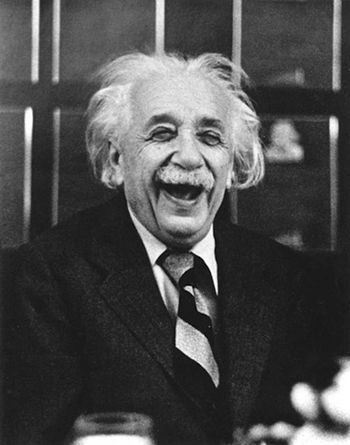
\includegraphics[width=0.7\textwidth]{figures/sample/einstein.jpeg}
		\caption{Figure 1}
		\label{fig_multienv_1}
	\end{subfigure}
	~
	\begin{subfigure}[t]{0.7\textwidth}
		\centering
		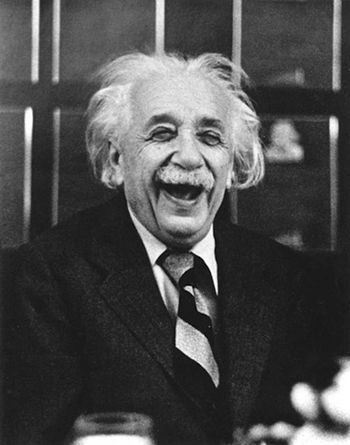
\includegraphics[width=0.7\textwidth]{figures/sample/einstein.jpeg}
		\caption{Figure 2}
		\label{fig_multienv_2}
	\end{subfigure}
	
	\caption{A Multi-Figure Environment}
	\label{fig_multienv}
\end{figure}

\section{Tables}

Here is a sample table (Table~\ref{tab_sample}):

	\begin{table}[ht]
	\centering
	\begin{tabular}{ m{0.2\textwidth} m {0.1\textwidth} m{0.15\textwidth} }
		\toprule
		A & $\longleftrightarrow$ & B \\
		C & $\longleftrightarrow$ & D \\
		\bottomrule	
	\end{tabular}	
	\caption{A sample table}	
	\label{tab_sample}
\end{table}

\subsection{Long Tables}
A sample long table is shown in Appendix~\ref{appendix_b}.

\section{Equations}

Here is a sample equation (Equation~\ref{eq_lineslope}):

\begin{equation} \label{eq_lineslope}
	y = mx + b
\end{equation}
       \setcounter{figure}{0}
       \setcounter{equation}{0}
       \setcounter{table}{0}

  \chapter{Conclusion}

Every thesis also needs a concluding chapter
        \setcounter{figure}{0}
        \setcounter{equation}{0}
        \setcounter{table}{0}

%--------------------Appendix-------------------------
\begin{appendix}
	\chapter{Your Appendix}
\label{appendix_a}

Your appendix goes here.

		\setcounter{figure}{0}
		\setcounter{equation}{0}
		\setcounter{table}{0}
		
	\chapter{Long Tables}
\label{appendix_b}

This appendix demonstrates the use of a long table that spans multiple pages.

\begin{center}
\begin{longtable}{P{3cm}P{3cm}P{2.5cm}P{3.5cm}}
\toprule
\hline
\textbf{Col A} & \textbf{Col B} & \textbf{Col C} & \textbf{Col D} \\ \midrule

\endfirsthead
\multicolumn{4}{c}{\textit{Continued from previous page}} \\ \hline
\textbf{Col A} & \textbf{Col B} & \textbf{Col C} & \textbf{Col D} \\ \hline
\endhead
\hline \multicolumn{4}{r}{\textit{Continued on the next page}} \\
\endfoot
\hline
\endlastfoot

A & B & C & D \\ \midrule

A & B & C & D \\ \midrule

A & B & C & D \\ \midrule

A & B & C & D \\ \midrule

A & B & C & D \\ \midrule

A & B & C & D \\ \midrule

A & B & C & D \\ \midrule

A & B & C & D \\ \midrule

A & B & C & D \\ \midrule

A & B & C & D \\ \midrule

A & B & C & D \\ \midrule

A & B & C & D \\ \midrule

A & B & C & D \\ \midrule

A & B & C & D \\ \midrule

A & B & C & D \\ \midrule

A & B & C & D \\ \midrule

A & B & C & D \\ \midrule

A & B & C & D \\ \midrule

A & B & C & D \\ \midrule

A & B & C & D \\ \midrule

\hline
\end{longtable}
\end{center}

		\setcounter{figure}{0}
		\setcounter{equation}{0}
		\setcounter{table}{0}
\end{appendix}

%--------------------Bibliography-------------------------
% The bibliography is set up to allow for multiple bib files
%\bibliographystyle{natbib} 
% https://www.overleaf.com/learn/latex/Natbib_citation_styles
% https://www.overleaf.com/learn/latex/Natbib_bibliography_styles

% check which bibliography style your department prefers
\bibliographystyle{abbrvnat}
%\setcitestyle{round} % to have parantheses around the in-text citation
% if you want to add number you can do so using \usepackage[sort, numbers]{natbib}
\bibliography{references/references_first, references/references_another}

\label{NumDocumentPages}

\end{document}
%----------------- Document Ended ------------------
